\documentclass[a4paper]{article}
\usepackage{amsmath, amssymb, amsthm}
\usepackage{fancyhdr}
\usepackage{enumitem}
\usepackage{physics}
\usepackage[english]{babel}
\usepackage{geometry}
\usepackage{graphicx}
\usepackage{hyperref}
\usepackage{mathrsfs}
\usepackage{epstopdf}
\usepackage{float}

\title{\textbf{Homework Of Gauge Theory}}
\author{Petrel of Sun}
\date{}

\begin{document}
\maketitle

\noindent \textbf{Question 1}
\par Pf:
\begin{align}
    &\textbf{1.}\left< y \right|e^{-i\hat{H}\delta t}\left| x \right> =\int{\frac{dp}{2\pi}e^{i\delta t[p\dot{q}-H]}}\\\nonumber
    \\ 
    &\textbf{2.}\int_{-\infty}^{\infty}{dxe^{-a(x-b)^2}}
    =\sqrt{\frac{\pi}{a}}\\\nonumber
    \\ 
    &\textbf{3.}\int_{-\infty}^{\infty}{dxf(x-b)}
    =\int_{-\infty}^{\infty}{dxf(x)}
\end{align}
\par
Whether it has always been established
\\ \\
\textbf{Sol:}
\par\textbf{1.}
\begin{equation}
    \begin{split}
       \left< y \right|e^{-i\hat{H}\delta t}\left| x \right> 
       &=e^{-iV(x)\delta t}\left<y\right|e^{-i\frac{\hat{p}^2}{2m}\delta t}\left| x \right> \\
       &=e^{-iV(x)\delta t}\left<y\right|e^{-i\frac{\hat{p}^2}{2m}\delta t}(\int{dp\left|p\right>\left<p\right|})\left| x \right> \\
       &=e^{-iV(x)\delta t}\int{dp e^{-i\frac{\hat{p}^2}{2m}\delta t}\left< y \mid p \right> \left< p \mid x \right>}\\
       &=e^{-iV(x)\delta t}\int{\frac{dp}{2\pi}e^{-i\frac{\hat{p}^2}{2m}\delta t}e^{ip(y-x)}}\\
       &=\int{\frac{dp}{2\pi}e^{i\delta t[p\frac{(y-x)}{\delta t}-(\frac{\hat{p}^2}{2m}+V(x))]}}
    \end{split}
\end{equation}
\par In which,
\par 
\begin{equation}
    \frac{y-x}{\delta t}=\dot{q}
\end{equation}
\begin{equation}
    \frac{\hat{p}^2}{2m}+V(x)=H
\end{equation}
\par p is generalized momentum, $\dot{q}$ is generalized velocity, and H is hamiltonian.
\par Finally, We can get,
\par \begin{equation}
     \left< y \right|e^{-i\hat{H}\delta t}\left| x \right> =\int{\frac{dp}{2\pi}e^{i\delta t[p\dot{q}-H]}}
\end{equation}

\par\textbf{2.}
By the translation invariance of the infinite integral, we can get,
\begin{equation}
\int_{-\infty}^{\infty}{dxe^{-a(x-b)^2}}
    =\int_{-\infty}^{\infty}{dxe^{-ax^2}}
\end{equation}
\par And then,
\begin{equation}
   \begin{split}
     (\int_{-\infty}^{\infty}{dxe^{-ax^2}})^2
    &=\int_{-\infty}^{\infty}{dxe^{-ax^2}}\int_{-\infty}^{\infty}{dye^{-ay^2}}\\
    &=\int_{-\infty}^{\infty}{dxdye^{-a(x^2+y^2)}}
  \end{split}
\end{equation}
\par In which, $x^2+y^2=r^2$, $dxdy=rdrd\theta$.
\par Substituting into Eq.(9) gives,
\begin{equation}
    \nonumber\int_{0}^{2\pi}{d\theta}\int_{0}^{\infty}{\frac{1}{2}dr^2 e^{-ar^2}}=\frac{\pi}{a}
\end{equation}
\par Finally,we can get,
\begin{equation}
    \int_{-\infty}^{\infty}{dxe^{-a(x-b)^2}}=\sqrt{\frac{\pi}{a}}
\end{equation}

\par\textbf{3.} The formula is not always valid. Need to be judged by the degree of divergence of the function $f(x)$. Generally, it can be applied directly.
\\
\\
\noindent \textbf{Question 2}
\par Pf:
\begin{equation}
    Z[J]=\sum_n{\frac{i^n}{n!}}\prod_{i}^{n}{\int{d
    ^4x_{i}J(x_{i})G^{(n)}(x_{1},x_{2},\cdot\cdot\cdot,x_{n})}}
\end{equation} 
\\ \\
\textbf{Sol:}
\par Generating function
\begin{equation}
Z[J]=\left<0\mid0\right>^J=\left<0\right|T\left\{e^{i\int{d^4xJ\varPhi}}\right\}\left|0\right>
\end{equation}
\par Based on the Dyson series,we can get,
\begin{equation}
\begin{split}
    T\left\{e^{i\int{d^4xJ\varPhi}}\right\}
    =&\sum_{n=0}^{\infty}{\frac{(-i)^n}{n!}\int{dt_{1}}\int{dt_{2}}\cdot\cdot\cdot\int{dt_{n}}}
    \\
    &\cdot{T\left\{[(J(x_{1})\varPhi(x_{1})][(J(x_{2})\varPhi(x_{2})]\cdot\cdot\cdot[(J(x_{n})\varPhi(x_{n})]\right\}}\\
    =&\sum_{n=0}^{\infty}{\frac{(-i)^n}{n!}\int{dt_{1}J(x_{1})}\int{dt_{2}J(x_{2})}\cdot\cdot\cdot\int{dt_{n}}J(x_{n})}
    \cdot\\
    &\cdot{T\left\{\varPhi(x_{1})\varPhi(x_{2})\cdot\cdot\cdot\varPhi(x_{n})\right\}}
\end{split}
\end{equation}
\par Substituting Eq.(13) into Eq.(12), we can get,
\begin{equation}
\begin{split}
    Z[J]=&\sum_{n=0}^{\infty}{\frac{(-i)^n}{n!}\int{dt_{1}J(x_{1})}\int{dt_{2}J(x_{2})}\cdot\cdot\cdot\int{dt_{n}}J(x_{n})}
    \cdot\\
    &\cdot\left<0\right|{T\left\{\varPhi(x_{1})\varPhi(x_{2})\cdot\cdot\cdot\varPhi(x_{n})\right\}}\left|0\right>\\
    =&\sum_{n=0}^{\infty}{\frac{(-i)^n}{n!}\int{dt_{1}J(x_{1})}\int{dt_{2}J(x_{2})}\cdot\cdot\cdot\int{dt_{n}}J(x_{n})G^{(n)}(x_{1},x_{2},\cdot\cdot\cdot,x_{n})}\\
    =&\sum_n{\frac{i^n}{n!}}\prod_{i}^{n}{\int{d
    ^4x_{i}J(x_{i})G^{(n)}(x_{1},x_{2},\cdot\cdot\cdot,x_{n})}}
\end{split}
\end{equation}
\\
\\
\noindent \textbf{Question 3}
\begin{equation}
    K(x,y)=\delta^{(4)}(x-y)(\partial^2+m^2-i\epsilon)=\int{\frac{d^4k}{(2\pi)^4}\Tilde{K}e^{-ik(x-y)}}
\end{equation}
\par In which $\Tilde{K}=-k^2+m^2$.
\begin{equation}
    i\Delta(x,y)=\int{\frac{d^4k}{(2\pi)^4}\frac{1}{-k^2+m^2}e^{-ik(x-y)}}
\end{equation}
\par  Check that $i\Delta$ is the inverse of K.
\begin{equation}
    \int{d^4zK(x,z)(i\Delta(z,y))}=\int{d^4z(i\Delta(x,z))K(z,y)}=\delta^{(4)}(x,y)
\end{equation}
\\ \\
\textbf{Sol:}
\begin{equation}
\begin{split}
    \int{d^4zK(x,z)(i\Delta(z,y))}=&\int{d^4z}\int{\frac{d^4k_{1}}{(2\pi)^4}(-k_{1}^2+m^2)e^{-ik_{1}(x-z)}}\\
    &\cdot\int{\frac{d^4k_{2}}{(2\pi)^4}\frac{1}{-k_{2}^2+m^2}e^{-ik_{2}(z-y)}}\\
    =&\int{\frac{d^4k_{1}}{(2\pi)^4}}\int{\frac{d^4k_{2}}{(2\pi)^4}\frac{-k_{1}^2+m^2}{k_{2}^2+m^2}e^{-ik_{1}x}e^{ik_{2}y}}\int{d^4ze^{i(k_{1}-k_{2})z}}\\
    =&\int{\frac{d^4k_{1}}{(2\pi)^4}}\int{\frac{d^4k_{2}}{(2\pi)^4}\frac{-k_{1}^2+m^2}{k_{2}^2+m^2}e^{-ik_{1}x}e^{ik_{2}y}}\cdot(2\pi)^4\delta^{(4)}(k_{1}-k_{2})\\
    =&\int{\frac{d^4k_{1}}{(2\pi)^4}e^{ik_{1}(y-x)}}\\
    =&\delta^{(4)}(y-x)=\delta^{(4)}(x,y)
\end{split}
\end{equation}
\par The same reasoning can be used to derive
\begin{equation}
    \int{d^4z(i\Delta(x,z))K(z,y)}=\delta^{(4)}(x,y)
\end{equation}
\\
\\
\noindent \textbf{Question 4}
\par 1. Free 4-point Green Functions,
\begin{equation}
    G_{0}^{(4)}=\Delta_{1,2}\Delta_{3,4}+\Delta_{1,3}\Delta_{2,4}+\Delta_{1,4}\Delta_{2,3}
\end{equation}
\par 2. Free n-point Green Functions,
\begin{equation}
    \begin{split}
        n=2m-1:& \quad 0\\
        n=2m:& \quad \frac{2m!}{m!2^m}
    \end{split}
\end{equation}
\\ \\
\textbf{Sol:}
\par\textbf{1. }Free 4-point Green Functions
\begin{equation}
    G_{0}^{(4)}=
    {\left< 0\right|T{\left\{\phi(x)\phi(y)\right\}}\left|0\right>}_{0}
    =\left.\frac{1}{Z_{0}[0]}\frac{\delta}{i\delta J(x_{1})}\frac{\delta}{i\delta J(x_{2})}\frac{\delta}{i\delta J(x_{3})}\frac{\delta}{i\delta J(x_{4})}Z_{0}[J]\right|_{J=0}
\end{equation}
\par We know that,
\begin{equation}
    Z_{0}[J]=\frac{Z_{0}[0]}{Z[0]}\sum_{n}\frac{(-1/2)^n}{n!}(J\Delta J)^n\
\end{equation}
\par In which $J\Delta J=\int{d^4xd^4yJ(x)\Delta(x,y) J(y)}$
\par We can get,
\begin{equation}
    \begin{split}
            &\frac{\delta}{\delta J(x_{1})}(\int{d^4xd^4yJ(x)\Delta(x,y) J(y)})^{n}\\
            &=n(\int{d^4xd^4yJ(x)\Delta(x,y) J(y)})^{n-1}\cdot(\int{d^4xd^4y\delta^{(4)}(x-x_{1})\Delta(x,y) J(y)}\\
            &+\int{d^4xd^4y\delta^{(4)}(y-x_{1})\Delta(x,y) J(x)})\\
            &=n(\int{d^4xd^4yJ(x)\Delta(x,y) J(y)})^{n-1}\cdot 2\int{d^4x\Delta(x,x_{1})J(x)}
    \end{split}
\end{equation}
\begin{equation}
    \begin{split}
        &\frac{\delta^2}{\delta J(x_{1})\delta J(x_{2})}(\int{d^4xd^4yJ(x)\Delta(x,y) J(y)})^{n}\\
        &=n(n-1)(\int{d^4xd^4yJ(x)\Delta(x,y) J(y)})^{n-2}\cdot 2\int{d^4x \Delta(x,x_{2}) J(x)}\\ 
        &\cdot2\int{d^4x \Delta(x,x_{1}) J(x)}+n(\int{d^4xd^4yJ(x)\Delta(x,y) J(y)})^{n-1}\cdot 2\Delta(x_{2},x_{1})\\
    \end{split}
\end{equation}
\begin{equation}
    \begin{split}
        &\frac{\delta^3}{\delta J(x_{1})\delta J(x_{2})\delta J(x_{3})}(\int{d^4xd^4yJ(x)\Delta(x,y) J(y)})^{n}\\
        &=n(n-1)(n-2)(\int{d^4xd^4yJ(x)\Delta(x,y) J(y)})^{n-3}\cdot 2\int{d^4x \Delta(x,x_{3}) J(x)}\\ 
        &\cdot 2\int{d^4x \Delta(x,x_{2}) J(x)}\cdot2\int{d^4x \Delta(x,x_{1}) J(x)}\\
        &+n(n-1)(\int{d^4xd^4yJ(x)\Delta(x,y) J(y)})^{n-2}\cdot 2 \Delta(x_{3},x_{2})\cdot2\int{d^4x \Delta(x,x_{1})J(x)}\\
        &+n(n-1)(\int{d^4xd^4yJ(x)\Delta(x,y) J(y)})^{n-2}\cdot 2 \Delta(x_{3},x_{1})\cdot2\int{d^4x \Delta(x,x_{2})J(x)}\\
        &+n(n-1)(\int{d^4xd^4yJ(x)\Delta(x,y) J(y)})^{n-2}\cdot2\int{d^4\Delta(x,x_{3})J(x)} \cdot2\Delta(x_{2},x_{1})\\
    \end{split}
\end{equation}
\begin{equation}
    \begin{split}
        &\frac{\delta^4}{\delta J(x_{1})\delta J(x_{2})\delta J(x_{3})\delta J(x_{4})}(\int{d^4xd^4yJ(x)\Delta(x,y) J(y)})^{n}\\
        &=n(n-1)(n-2)(n-3)(\int{d^4xd^4yJ(x)\Delta(x,y) J(y)})^{n-4}\cdot 2\int{d^4x \Delta(x,x_{4}) J(x)}\\
        &\cdot 2\int{d^4x \Delta(x,x_{3}) J(x)}\cdot 2\int{d^4x \Delta(x,x_{2}) J(x)}\cdot2\int{d^4x \Delta(x,x_{1}) J(x)}\\
        &+n(n-1)(n-2)(\int{d^4xd^4yJ(x)\Delta(x,y) J(y)})^{n-3}\cdot 2\Delta(x_{4},x_{3})\\ 
        &\cdot 2\int{d^4x \Delta(x,x_{2}) J(x)}\cdot2\int{d^4x \Delta(x,x_{1})J(x)}\\
        &+n(n-1)(n-2)(\int{d^4xd^4yJ(x)\Delta(x,y) J(y)})^{n-3}\cdot 2\Delta(x_{4},x_{2})\\ 
        &\cdot 2\int{d^4x \Delta(x,x_{3}) J(x)}\cdot2\int{d^4x \Delta(x,x_{1})J(x)}\\
        &+n(n-1)(n-2)(\int{d^4xd^4yJ(x)\Delta(x,y) J(y)})^{n-3}\cdot 2\Delta(x_{4},x_{1})\\ 
        &\cdot 2\int{d^4x \Delta(x,x_{3}) J(x)}\cdot2\int{d^4x \Delta(x,x_{2})J(x)}\\
        &+n(n-1)(n-2)(\int{d^4xd^4yJ(x)\Delta(x,y) J(y)})^{n-3}\int{d^4x \Delta(x,x_{4})J(x)}\\
        &\cdot 2 \Delta(x_{3},x_{2})\cdot2\int{d^4x \Delta(x,x_{1})J(x)}\\
        &+n(n-1)(\int{d^4xd^4yJ(x)\Delta(x,y) J(y)})^{n-2}\cdot 2 \Delta(x_{3},x_{2})\cdot2 \Delta(x_{4},x_{1})\\
        &+n(n-1)(n-2)(\int{d^4xd^4yJ(x)\Delta(x,y) J(y)})^{n-3}\int{d^4x \Delta(x,x_{4})J(x)}\\
        &\cdot 2 \Delta(x_{3},x_{1})\cdot2\int{d^4x \Delta(x,x_{2})J(x)}\\
        &+n(n-1)(\int{d^4xd^4yJ(x)\Delta(x,y) J(y)})^{n-2}\cdot 2 \Delta(x_{3},x_{1})\cdot2 \Delta(x_{4},x_{2})\\
        &+n(n-1)(n-2)(\int{d^4xd^4yJ(x)\Delta(x,y) J(y)})^{n-3}\cdot2\int{d^4\Delta(x,x_{4})J(x)}\\
        &\cdot2\int{d^4\Delta(x,x_{3})J(x)}\cdot2\Delta(x_{2},x_{1})\\
        &+n(n-1)(\int{d^4xd^4yJ(x)\Delta(x,y) J(y)})^{n-2}\cdot2\Delta(x_{4},x_{3}) \cdot2\Delta(x_{2},x_{1})\\
    \end{split}
\end{equation}
\par Substitute into Eq.(22),We can get,
\begin{equation}
    \begin{split}
        G_{0}^{(4)}&=\Delta(x_{3},x_{2})\Delta(x_{4},x_{1})+\Delta(x_{3},x_{1})\Delta(x_{4},x_{2})+\Delta(x_{4},x_{3})\Delta(x_{2},x_{1})\\
        &=\Delta_{3,2}\Delta_{4,1}+\Delta_{3,1}\Delta_{4,2}+\Delta_{4,3}\Delta_{2,1}
    \end{split}
\end{equation}
\par \textbf{2.} According to Eq.(23),the term in $Z_{0}[J]$ is even power of $J$. For $G_{0}^{(n)}$,if $n=2m-1$, the $k$th term of the function is $(2(k-m)+1)$th power of $J$, in which $k=0,1,2,\cdots$. When $n$ takes odd power,there is no 0th power in $G_{0}^{(n)}$,the function equal to 0 because $J$ need to be 0 in the end.
\par If $n=2m$, the $k$th term of the function is $2(k-m)$th power of $J$, $k=0,1,2,\cdots$. So there are 0th terms in $G_{0}^{(n)}$ when $k=m$. The final form of $G_{0}^{(n)}$ is composed of two-point correlation function $\Delta$, and each term of $G_{0}^{(n)}$ will take all n points.Note that here these $\Delta$ functions can be interchanged.
\par We take two point every times as variables of the $\Delta$ function, until takes all $n=2m$ points. Let these $\Delta$ function mutiply, We can get one term of $G_{0}^{(n)}$. By this way, we can get the numbers of different terms,
\begin{equation}
    C_{n}^2 C_{n-2}^2\cdots C_{n-2i}^2 \cdots C_{2}^2=\frac{n!}{2^m}
\end{equation}
\par However, this way of taking points does not take into account that $\Delta$ functions can be interchanged. So each terms has $m!$ repetitions in the above way. Actually, we get the numbers of different terms,
\begin{equation}
    \frac{(2m)!}{m!2^m}
\end{equation}
\\
\\
\noindent \textbf{Question 5}
\par \textbf{1.} Get the Feynman Rules for the following Lagrangian.
\begin{equation}
    \mathcal{L}=\frac{1}{2}(\partial\Phi)^2-\frac{1}{2}m^2\Phi^2-\frac{\lambda}{3!}\Phi^3
\end{equation}
\par \textbf{2.} Treat $m^2$ as perturbation, get the Feynman Rules for the Lagragian.
\begin{equation}
    \mathcal{L}=\frac{1}{2}(\partial\Phi)^2-\frac{1}{2}m^2\Phi^2
\end{equation}
\par \textbf{3.} Draw the Feynman diagram(s) and write down the corresponding amplitude(s) for the process $\phi\phi\to\phi\phi$ up to $\lambda^2$ order.
\begin{equation}
    \begin{split}
        \mathcal{M}&=\frac{\lambda^2}{2}\int{\frac{d^4q}{(2\pi)^4}\frac{1}{(q^2-m^2)[(q-k_{1}-k_{2})^2-m^2]}}\\
        &+\frac{1}{(q^2-m^2)[(q+p_{2}-k_{2})^2-m^2]}+\frac{1}{(q^2-m^2)[(q+p_{2}-k_{1})^2-m^2]}
    \end{split}
\end{equation}
\\ \\
\textbf{Sol:}
\par\textbf{1.} The generating function with interaction term(s),
\begin{equation}
    Z(J)=exp(i\int{d^4x\mathcal{L}_{I}(\frac{\delta}{i\delta J(x)})})Z_{0}(J)
\end{equation}
\par The interaction term takes $\mathcal{L}_{I}=-\frac{\lambda}{3!}\Phi^3$. We do a Taylor expansion about $-i\frac{\lambda}{3!}$ for the e-index, and retain up to the second-order term,
\begin{equation}
    \begin{split}
            exp(-i\int{d^4x\frac{\lambda}{3!}(\frac{\delta}{i\delta J(x)})^3})
            &=\sum{\frac{1}{n!}[\int{d^4x(\frac{\delta}{i\delta J(x)})^3}]^{n}(-i\frac{\lambda}{3!})^{n}}\\
            &=1-i\frac{\lambda}{3!}\int{d^4x(\frac{\delta}{i\delta J(x)})^3}+\mathcal{O}(\lambda^2)
    \end{split}
\end{equation}  
\par Substitute Eq.(35) into Eq.(34), we can get,
\begin{equation}
        Z(J)=Z_{0}(J)+\frac{\lambda}{3!}\int{d^4x[(\frac{\delta}{\delta J(x)})^3Z_{0}(J)]}+\mathcal{O}(\lambda^2)\\
\end{equation}
\par Now, we calculate the second term,
\begin{equation}
    \begin{split}
        (\frac{\delta}{\delta J(x)})^3Z_{0}(J)
        &=A(\frac{\delta}{\delta J(x)})^3[\sum_{n=0}{\frac{(-1/2)^n}{n!}(J\Delta J)^n}]\\
        &=A(\frac{\delta}{\delta J(x)})^3[1-\frac{1}{2}J\Delta J+\sum_{n=2}{\frac{(-1/2)^{n}}{n!}(J\Delta J)^n}]
    \end{split}
\end{equation}
According to Eq.(25)(26)(27), we can get, 
\begin{equation}
    (\frac{\delta}{\delta J(x)})^3(J\Delta J)=0
\end{equation}
And $n\ge2$
\begin{equation}
    \begin{split}
        &(\frac{\delta}{\delta J(x)})^3(J\Delta J)^n\\
        &=n(n-1)(n-2)(\int{d^4x_{1}d^4x_{2}J(x_{1})\Delta(x_{1},x_{2}) J(x_{2})})^{n-3}\cdot [2\int{d^4x_{1} \Delta(x_{1},x) J(x_{1})}]^3\\ 
        &+3n(n-1)(\int{d^4x_{1}d^4x_{2}J(x_{1})\Delta(x_{1},x_{2}) J(x_{2})})^{n-2}\cdot 2 \Delta(x,x)\cdot2\int{d^4x_{1} \Delta(x_{1},x)J(x_{1})}\\
    \end{split}
\end{equation}
\par Substitute Eq.(38)(39)(40) into Eq.(37), we can get,
\begin{equation}
    \begin{split}
         &(\frac{\delta}{\delta J(x)})^3Z_{0}(J)\\
         &=A\sum_{n=2}\frac{(-1/2)^n}{n!}(\frac{\delta}{\delta J(x)})^3(J\Delta J)^n\\
         &=3A\sum_{n=2}\frac{(-1/2)^{n-2}}{(n-2)!}(J\Delta J)^{n-2}\Delta(x,x)\int{d^4x_{1}\Delta(x_{1},x)J(x_{1})}\\
         &-A\sum_{n=3}\frac{(-1/2)^{n-3}}{(n-3)!}(J\Delta J)^{n-3}[\int{d^4x_{1}\Delta(x_{1},x)J(x_{1})}]^3\\
         &=3Z_{0}(J)\Delta(x,x)\int{d^4x_{1}\Delta(x_{1},x)J(x_{1})}-Z_{0}(J)[\int{d^4x_{1}\Delta(x_{1},x)J(x_{1})}]^3\\
    \end{split}
\end{equation}
\par Finally, we get the generating function with interaction terms,
\begin{equation}
    \begin{split}
        Z(J)=&Z_{0}(J)\left\{1+\frac{\lambda}{2}\int{d^4x\Delta(x,x)\int{d^4x_{1}\Delta(x_{1},x)J(x_{1})}}\right.\\
         &\left.-\frac{\lambda}{3!}\int{d^4x[\int{d^4x_{1}\Delta(x_{1},x)J(x_{1})}]^3}\right\}\\
         =&Z_{0}(J)\cdot Z_{I}(J)
    \end{split}
\end{equation}
\par n-point Green function,
\begin{equation}
    G^{(n)}=\left.\left<T\left\{\Phi_{1}\Phi_{2}\cdots\Phi_{n}\right\}\right>=\frac{(-i)^n}{Z[0]}\frac{\delta^n}{\delta J_{1}\delta J_{2}\cdots\delta J_{n}}Z[J]\right|_{J=0}
\end{equation}
\par Using Eq.(43)(42), we can get one-point Green function,
\begin{equation}
    \begin{split}
        G^{(1)}&=\left.\frac{-i}{Z[0]}\frac{\delta}{\delta J(y_{1})}Z[J]\right|_{J=0}\\
        &=-\frac{i\lambda}{2}\int{d^4x \Delta(y_{1},x)\Delta(x,x)}
    \end{split}
\end{equation}
\par Using a line to represent the propagator, the two ends of the line are the two variables of the propagator represented by points, we can get,
\begin{figure}[h]
    \centering
    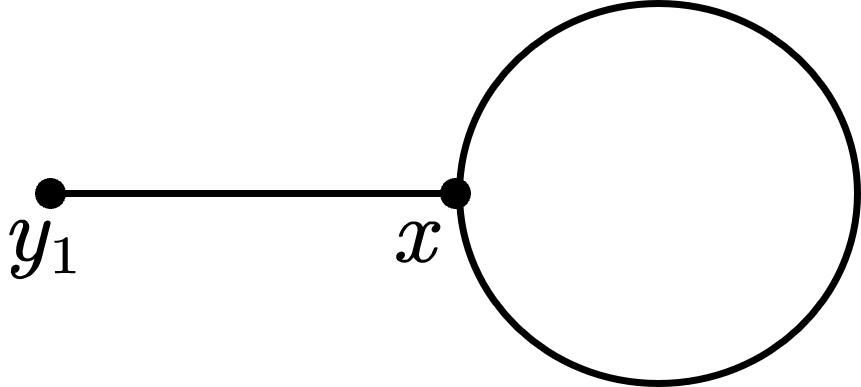
\includegraphics[width=0.4\linewidth]{1point.png}
    \caption{one-point diagram with interaction term}
    \label{fig:enter-label}
\end{figure}
\par Two-point Green function,
\begin{equation}
    \begin{split}
         G^{(2)}&=\left.-\frac{1}{Z[0]}\frac{\delta^2}{\delta J(y_{1})\delta J(y_{2})}Z[J]\right|_{J=0}\\
         &=\Delta(y_{1},y_{2})
    \end{split}
\end{equation}
\par Diagram represented as,
\begin{figure}[h]
    \centering
    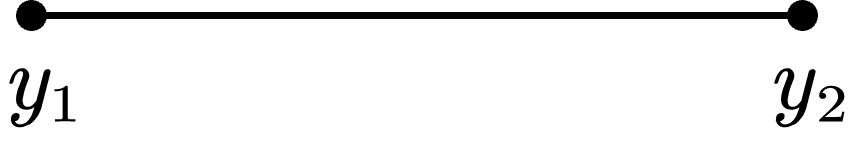
\includegraphics[width=0.3\linewidth]{2point.png}
    \caption{two-point diagram with interaction term}
    \label{fig:enter-label}
\end{figure}
\par Three-point Green function,
\begin{equation}
    \begin{split}
        G^{(3)}&=\left.\frac{i}{Z[0]}\frac{\delta^3}{\delta J(y_{1})\delta J(y_{2})\delta J(y_{3})}Z[J]\right|_{J=0}\\
         &=-\frac{i\lambda}{2}[\Delta(y_{2},y_{3})\int{d^4x \Delta(y_{1},x)\Delta(x,x)}+\Delta(y_{1},y_{3})\int{d^4x \Delta(y_{2},x)\Delta(x,x)}\\
         &+\Delta(y_{1},y_{2})\int{d^4x \Delta(y_{3},x)\Delta(x,x)}]-i\lambda\int{\Delta(y_{1},x)\Delta(y_{2},x)\Delta(y_{3},x)}
    \end{split}
\end{equation}
\par Diagram represented as,
\begin{figure}[H]
    \centering
    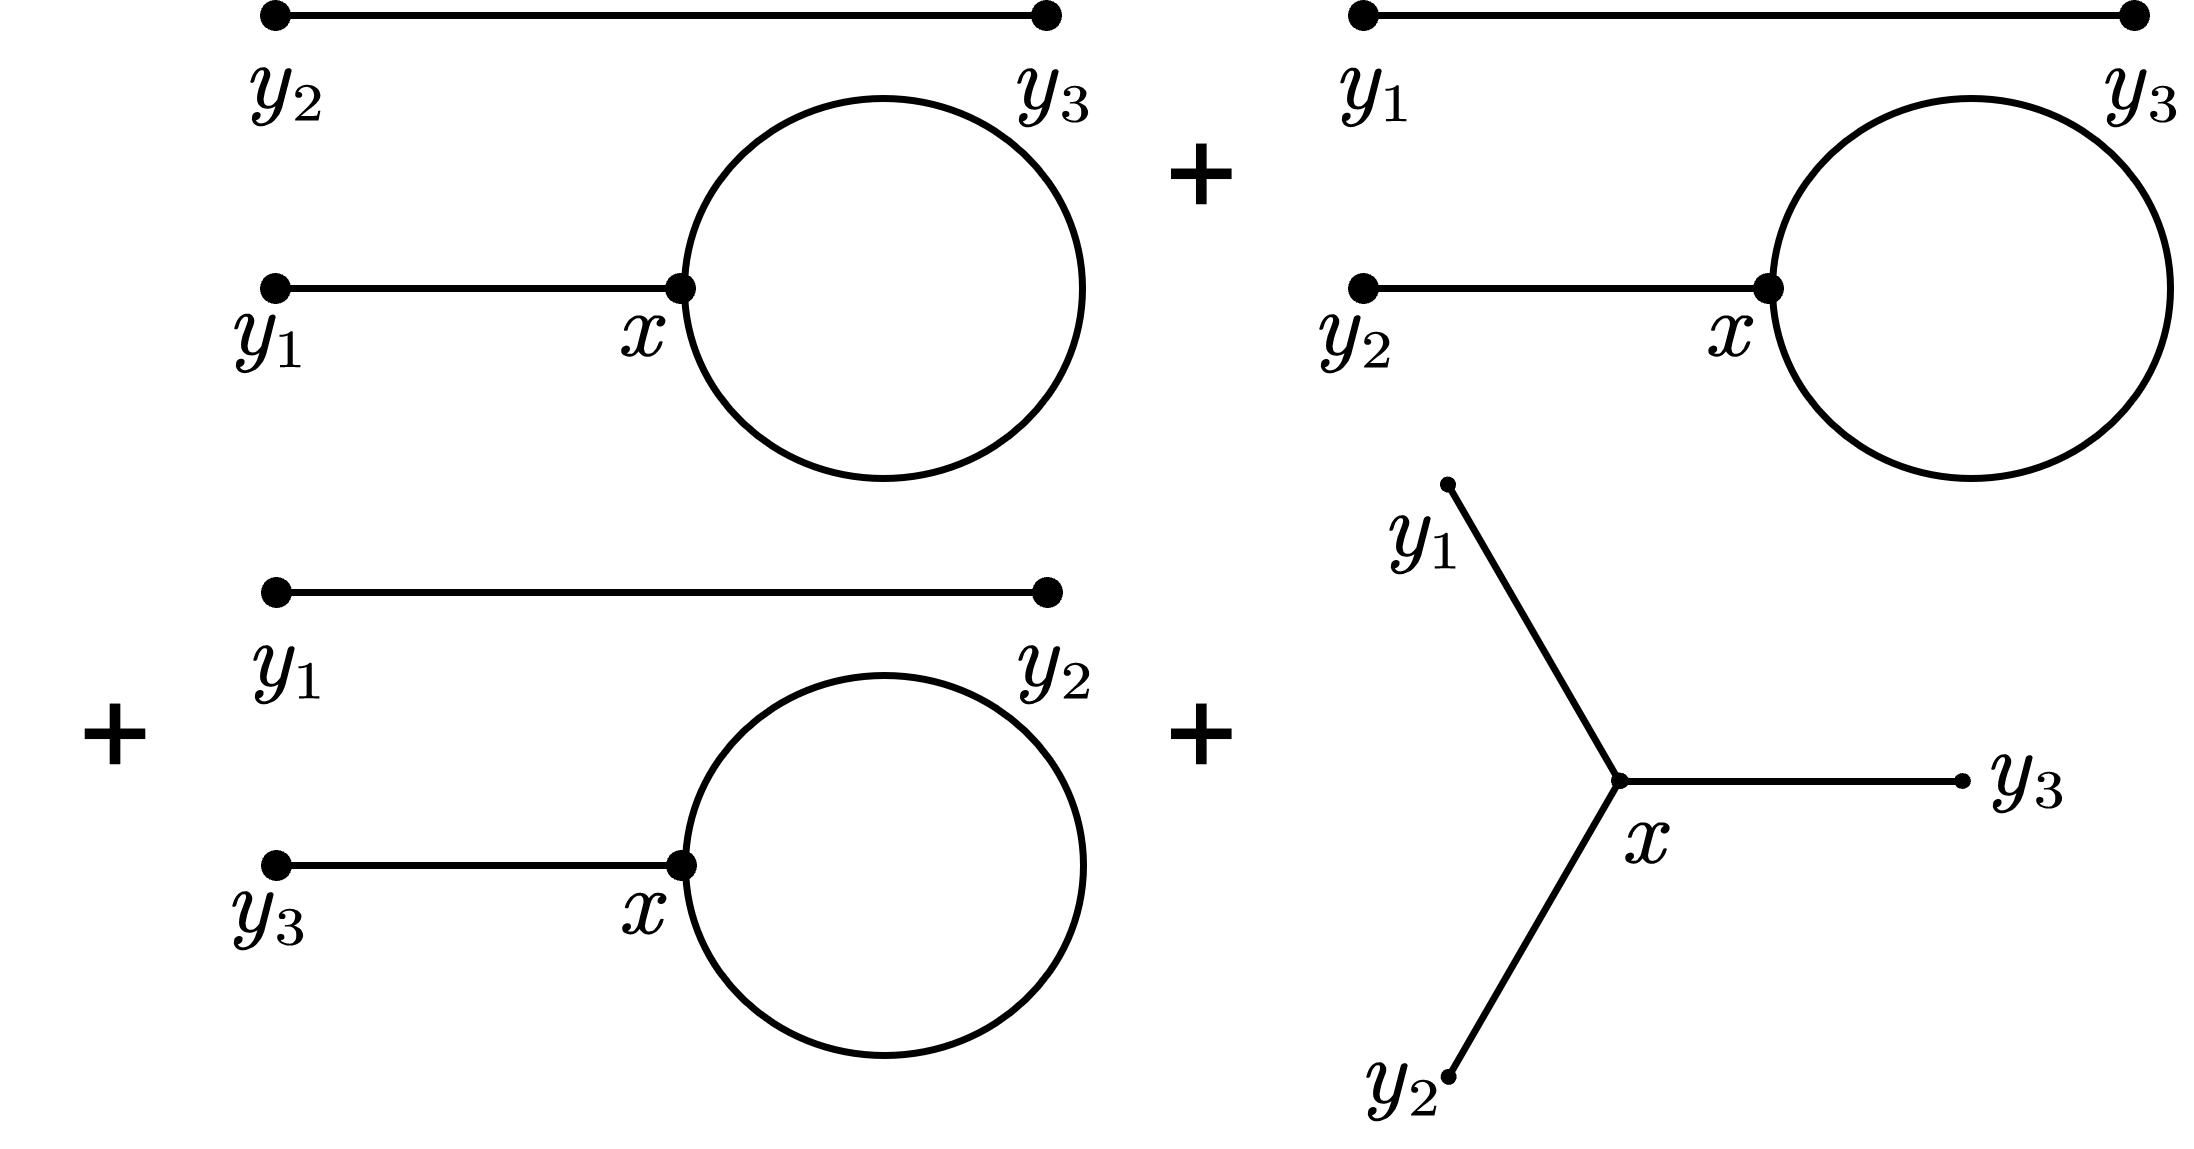
\includegraphics[width=0.8\linewidth]{3point.png}
    \caption{three-point diagram with interaction term}
    \label{fig:enter-label}
\end{figure}

\par In summary, we understand $\Delta$ as pagators, which connect $y_{i}$ with $y_{j}$ or $x$. $y_{i}$ point as the external points, which are determined by the particles in the initial and final states. And $x$ as the internal vertex, requires integration over the positions. The number of internal vertex is determined by the order of perturbative.
\end{document}









